% Womelsdorf Lab burst library user guide - Overview
% Written by Christopher Thomas.

\chapter{Overview}
\label{sect-over}

%
%
%
\section{Introduction}
\label{sect-over-intro}

Neural signals often contain transient oscillations in the local field
potential (``oscillatory bursts''). These represent coordinated activity of
many neurons. There is evidence that oscillatory bursts are correlated with
changes in connectivity within the brain and with certain types of data
processing, so identifying and characterizing these bursts in neural
recordings is useful.

An illustration of burst events within a neural signal is shown in Figure
\ref{fig-intro-burst}.
\figdef{%
\begin{center}
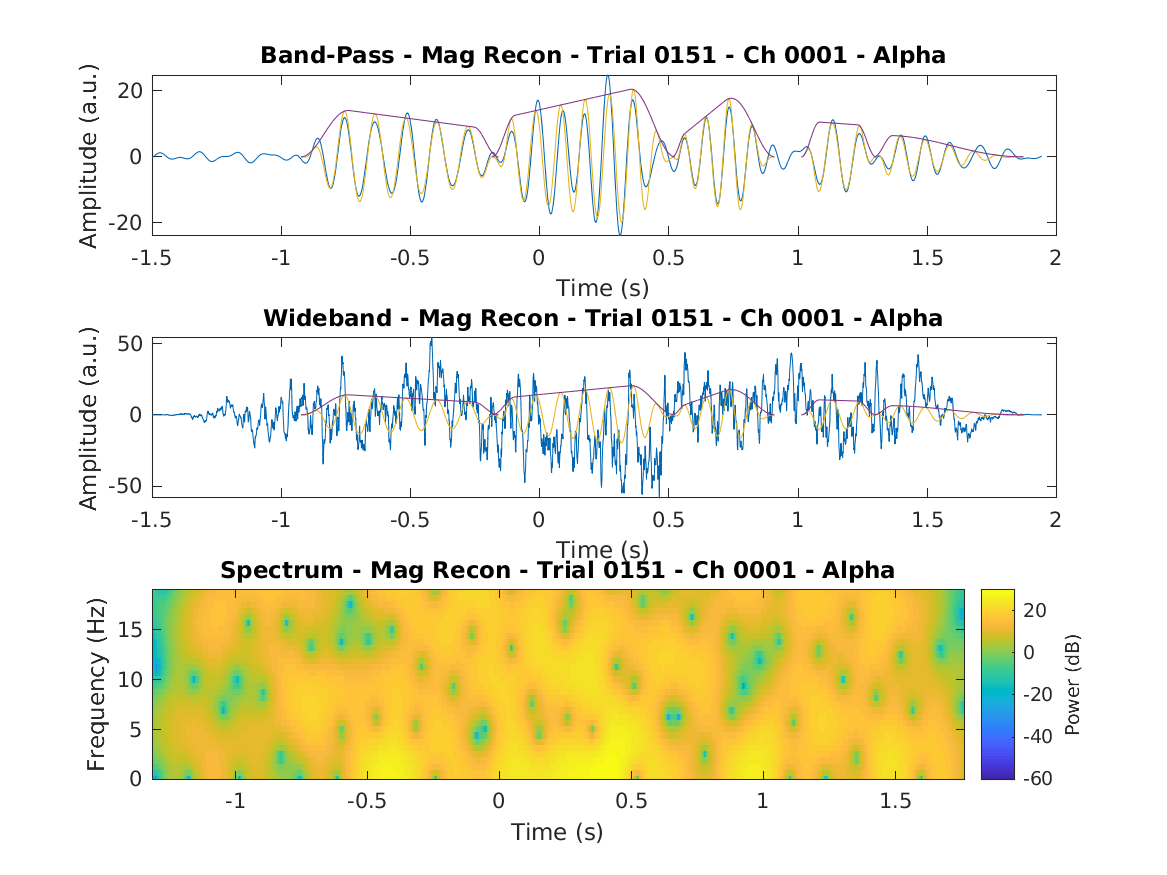
\includegraphics[height=3in]{plots2/commonwb-mag-tr0151-ch0001-al.png}
\end{center}
}{Neural waveform with burst events.}{fig-intro-burst}

The purpose of the wlBurst library is to provide the tools needed to identify
and characterize oscillatory bursts.

%
%
%
\section{The wlBurst Library}
\label{sect-over-lib}

The wlBurst library primarily uses the following types of data structure:

\begin{itemize}
%
\item \textbf{``Data traces''} are one-dimensional arrays containing
waveform samples.
%
\item \textbf{``Event lists''} are one-dimensional arrays containing
``event records'' (per \texttt{EVENTFORMAT.txt}). These are parametric
descriptions of oscillation events extracted from a data trace.
%
\item \textbf{``Field Trip data structures''} are structures of type
\texttt{ft\_datatype\_raw} produced by the Field Trip toolset. The wlBurst
library treats trial data within a FT data structure as a two-dimensional
array of data traces (indexed by trial number and channel number).
%
\item \textbf{``Event matrix''} structures are three-dimensional arrays
of event lists, describing events detected within a Field Trip data structure
indexed by frequency band, trial number, and channel number. A considerable
amount of auxiliary data is stored as well (per \texttt{EVMATRIX.txt}).

Event matrices may be converted to Field Trip data structures, to allow
the use of the Field Trip suite's visualization tools. This stores events
as individual FT trials. Information mapping events to the original band,
trial, and channel numbers is stored in the \texttt{trialinfo} structure,
and additional metadata is stored in a ``\texttt{wlnotes}'' structure
per \texttt{WLNOTES.txt}.
%
\end{itemize}

Library functions are divided into the following categories:

\begin{itemize}
%
\item \textbf{``Processing''} functions (in \texttt{lib-wl-proc})
perform segmentation, feature extraction, and other operations on single
data traces. Events are returned as ``event lists'', which can be further
manipulated.
%
\item \textbf{``Field Trip''} functions (in \texttt{lib-wl-ft})
perform event detection and other operations on Field Trip raw data
structures. Events detected are returned as ``event matrices'', which can
be further manipulated.
%
\item \textbf{``Synthesis''} functions (in \texttt{lib-wl-synth})
construct simulated neural recordings containing oscillation events,
providing data with known ground-truth.
%
\item \textbf{``Auxiliary''} functions (in \texttt{lib-wl-aux})
perform manipulations that don't fall into the previous categories.
%
\item \textbf{``Plotting''} functions (in \texttt{lib-wl-plot})
produce rough plots of various types of data. The output is generally not
publication-quality.
%
\end{itemize}

Library functions are documented in detail in the ``Function Reference''
document.

%
% This is the end of the file.
